\chapter{اللاجرانجيات والحقول وعمليات الجسيمات المحلية}

حقول البوزونات وحقول الفرميونات والحقل الكهرومغناطيسي كلها تخضع لمعادلات ذات طابع موجي. وتتضمن تلك المعادلات الحقول نفسها إلى جانب مشتقاتها المكانية والزمانية. ويمكن للمرء أن يسرد معادلة حركة منفصلة لكل حقل، لكن اللاجرانجي يجمع المنظومة بأكملها في تعبير مدمج واحد. ويعطي تطبيق قاعدة أويلر--لاجرانج على ذلك التعبير معادلات جميع الحقول دفعة واحدة.

هذا البناء يرتبط ارتباطًا وثيقًا بالفعل الساكن. والمهمة المباشرة هنا أكثر تحديدًا: تحديد ما الذي يعتمد عليه لاجرانجي الحقل، واستخدامه لاستخراج بضع معادلات كلاسيكية، ثم إعادة تفسير تعابير الحقول نفسها تفسيرًا كموميًا. وفي النظرية الكمومية يحكم اللاجرانجي حركة الجسيمات وتآثرها، وفي نهاية المطاف سعات التصادمات ومقاطعها العرضية.

\section{ترميز مدمج لمعادلات الحقول}

لحقل قياسي واحد، تعتمد الكثافة اللاجرانجية على الحقل وعلى مشتقاته الأولى،
\begin{equation}
\mathcal L
=
\mathcal L\!\left(\phi,\partial_t\phi,\partial_x\phi,\ldots\right)
=
\mathcal L\!\left(\phi,\partial_\mu\phi\right).
\end{equation}
وغالبًا ما تكون القائمة الصريحة للمشتقات الزمانية والمكانية أكثر فائدة أثناء الحساب؛ أمّا الترميز \(\partial_\mu\phi\) فيجمع القائمة نفسها في صيغة نسبية.

\begin{figure}[htbp]
\centering
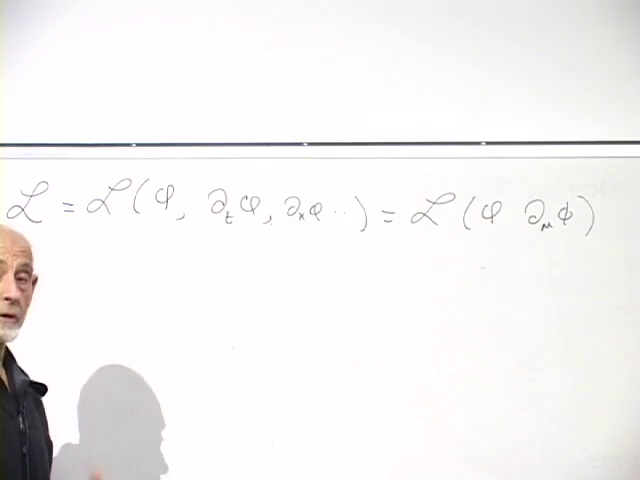
\includegraphics[width=0.82\textwidth]{lecture_09_figure_03.png}
\caption{اعتماد لاجرانجي لحقل قياسي على الحقل وعلى مشتقاته الزمكانية.}
\lectureframe{00:03:56}
\end{figure}

ومعادلة أويلر--لاجرانج للحقل هي
\begin{equation}
\frac{\partial}{\partial t}
\frac{\partial\mathcal L}{\partial\dot\phi}
+
\frac{\partial}{\partial x}
\frac{\partial\mathcal L}{\partial\phi_x}
+
\frac{\partial}{\partial y}
\frac{\partial\mathcal L}{\partial\phi_y}
+
\frac{\partial}{\partial z}
\frac{\partial\mathcal L}{\partial\phi_z}
=
\frac{\partial\mathcal L}{\partial\phi},
\end{equation}
حيث
\begin{equation}
\dot\phi=\frac{\partial\phi}{\partial t},
\qquad
\phi_x=\frac{\partial\phi}{\partial x},
\qquad
\phi_y=\frac{\partial\phi}{\partial y},
\qquad
\phi_z=\frac{\partial\phi}{\partial z}.
\end{equation}
وإذا كانت \(\mathcal L\) تتضمن عدة حقول، فتُطبَّق هذه القاعدة مرة واحدة على كل حقل. والنتيجة هي منظومة معادلات الحركة.

وأبسط مثال لحقل قياسي هو
\begin{equation}
\begin{split}
\mathcal L
&=
\frac12\dot\phi^2
-\frac12\phi_x^2
-\frac12\phi_y^2
-\frac12\phi_z^2
-V(\phi)
\\
&=
\frac12\dot\phi^2-\frac12(\boldsymbol\nabla\phi)^2-V(\phi).
\end{split}
\end{equation}
وتحمل حدود المشتقات المكانية إشارة معاكسة لإشارة حد المشتقة الزمنية. وبالتفاضل حدًا حدًا نحصل على
\begin{align}
\frac{\partial\mathcal L}{\partial\dot\phi}&=\dot\phi,
&
\frac{\partial\mathcal L}{\partial\phi_i}&=-\phi_i,
&
\frac{\partial\mathcal L}{\partial\phi}&=-V'(\phi),
\end{align}
ولذلك
\begin{equation}
\ddot\phi-\nabla^2\phi=-V'(\phi).
\end{equation}

\begin{figure}[htbp]
\centering
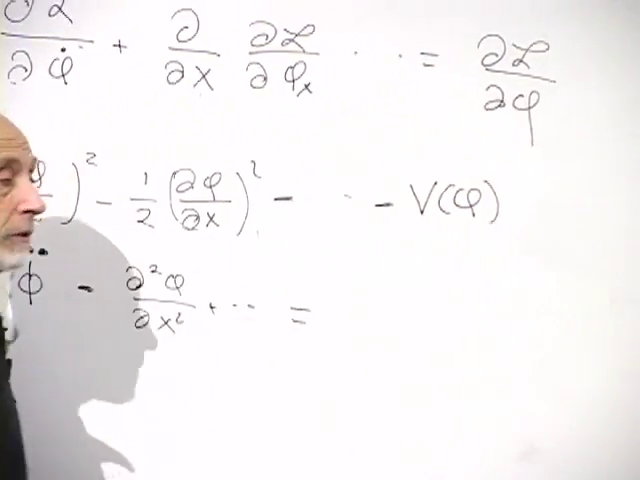
\includegraphics[width=0.74\textwidth]{lecture_09_figure_04.png}
\caption{معادلة أويلر--لاجرانج، ولاجرانجي الحقل القياسي، ومعادلة الحقل التي يولدها \(V(\phi)\).}
\lectureframe{00:08:23}
\end{figure}

هذه هي المعادلة التي يولدها لاجرانجي الحقل القياسي.\editorialnote{الإطار المحتفَظ به مقصوص عند الحافة اليسرى؛ والإكمال المعروض يحدده الاشتقاق الشفهي المحيط به مباشرة.}

هنا \(V(\phi)\) هي كثافة طاقة الوضع للحقل. وليس لمساهمة ثابتة في \(V\) أي أثر في هذه المعادلة لأن مشتقتها تنعدم. وجهد خطي ممكن جبريًا، لكنه لا يملك حدًا أدنى: إذ يمكن لطاقة الحقل أن تنحدر نحو سالب ما لا نهاية. لذلك فإن أول مثال مستقر هو
\begin{equation}
V(\phi)=\frac12m^2\phi^2,
\qquad
V'(\phi)=m^2\phi,
\end{equation}
الذي يعطي
\begin{equation}
\ddot\phi-\nabla^2\phi=-m^2\phi.
\end{equation}

ولإبراز معنى \(m\)، نعوّض بموجة مستوية،
\begin{equation}
\phi(\mathbf x,t)=\phi_0e^{i\omega t-i\mathbf k\cdot\mathbf x}.
\end{equation}
وعندئذ
\begin{equation}
\ddot\phi=-\omega^2\phi,
\qquad
\nabla^2\phi=-\mathbf k^2\phi,
\end{equation}
فتصبح معادلة الموجة
\begin{equation}
-\omega^2\phi+\mathbf k^2\phi=-m^2\phi.
\end{equation}
وبعد اختزال \(\phi\)،
\begin{equation}
\omega^2=\mathbf k^2+m^2.
\end{equation}
وفي وحدات يكون فيها \(\hbar=c=1\)، يكون التردد طاقة ويكون العدد الموجي زخمًا. ومن ثم
\begin{equation}
E^2=\mathbf p^2+m^2,
\end{equation}
أو، بعد إعادة قوى \(c\)، \(E^2=\mathbf p^2c^2+m^2c^4\). والمعلمة \(m\) هي كتلة كمّ واحد من الحقل.

يمكن فرض الثبات النسبي على مستوى الصياغة الموجزة. فإذا كانت \(\mathcal L\) كميةً قياسية لورنتزية، كانت معادلات حركتها ثابتةً تحت تحولات لورنتز. والإشارة النسبية بين المشتقات الزمنية والمكانية هي إشارة الزمكان المألوفة في النسبية الخاصة.

\section{اللاخطية والحقول الكلاسيكية المقترنة}

تُدخل الأسس الأعلى للحقل نوعًا جديدًا من السلوك. فإذا كان
\begin{equation}
V(\phi)=\frac12m^2\phi^2+g\phi^3,
\end{equation}
فإن
\begin{equation}
\ddot\phi-\nabla^2\phi=-m^2\phi-3g\phi^2.
\end{equation}
تعطي الحدود التربيعية في اللاغرانجي معادلات خطية في الحقل. أما الحدود التكعيبية وما فوقها فتعطي معادلات لاخطية.

يظهر هذا التمييز في حركة الحزم الموجية. ففي معادلة خطية، يمكن جمع حزمة متحركة نحو اليمين وحزمة متحركة نحو اليسار لتكوين حل آخر. وهما تتراكبان وتتداخلان مدةً من الزمن، ثم تمر كل منهما خلال الأخرى وتخرجان بأشكالهما الأصلية. أما مع الحدود اللاخطية، فتؤثر الحزم بعضها في بعض. ويمكنها أن تتشتت، أو تتشوه، أو تتفكك إلى موجات أشد تعقيدًا. والتداخل المؤقت للموجات الخطية ليس تفاعلًا؛ أما التغير الدائم في الحزم فيدل على اللاخطية.

يظهر النمط نفسه مع حقلين قياسيين. لنأخذ
\begin{align}
\mathcal L
&=
\frac12(\partial_\mu\phi)(\partial^\mu\phi)
+\frac12(\partial_\mu\rho)(\partial^\mu\rho)
-V(\phi,\rho),
\\
V(\phi,\rho)
&=
\frac12m^2\phi^2+\frac12M^2\rho^2+\rho\phi^2.
\end{align}
ومن دون الحد الأخير تكون المعادلتان مستقلتين،
\begin{equation}
\ddot\phi-\nabla^2\phi=-m^2\phi,
\qquad
\ddot\rho-\nabla^2\rho=-M^2\rho.
\end{equation}
وهما تصفان كمّات من نوعين، كتلتهما \(m\) و\(M\). ومع إدراج الحد المختلط،
\begin{align}
\ddot\phi-\nabla^2\phi&=-m^2\phi-2\rho\phi,
\\
\ddot\rho-\nabla^2\rho&=-M^2\rho-\phi^2.
\end{align}
تحتوي كل معادلة الآن على الحقل الآخر. فالمعادلتان مقترنتان ولاخطيّتان: إذ تبعثر حزمة \(\phi\) حزمة \(\rho\)، والعكس بالعكس. وتحكم حدود المشتقات علاقة الطاقة--الزخم، وتحدد الحدود التربيعية غير المشتقة الكتل، ويحمل الحد المختلط الأعلى رتبةً التفاعل. وهذا هو النمط الكلاسيكي الأساسي.

\section{حقول ديراك واقتران قياسي}

بالنسبة إلى حقل ديراك، تكون المعادلة من الرتبة الأولى في الزمن. وفي اختزال أحادي البعد، مع فهم الامتداد إلى ثلاثة اتجاهات مكانية، تكون بنية حدوده كما يلي
\begin{equation}
i\dot\Psi
\simeq
i\alpha\frac{\partial\Psi}{\partial x}+m\beta\Psi,
\qquad
i\boldsymbol\alpha\cdot\boldsymbol\nabla\Psi
=i\sum_i\alpha_i\frac{\partial\Psi}{\partial x_i}.
\end{equation}
وتؤثر المصفوفات \(\alpha_i\) و\(\beta\) في مركبات \(\Psi\). ويحتوي لاغرانجي مناظر على حد خطي في \(\partial_t\Psi\)، وحد ثنائي خطي في المشتقة المكانية يتضمن \(\alpha_i\)، وحد الكتلة الثنائي الخطي \(m\Psi^\dagger\beta\Psi\). ولا نحتاج هنا إلا إلى هذه الحقيقة البنيوية.\editorialnote{تُركت الإشارات والأقواس وموضع \(i\) في الصياغة المقترحة للاغرانجي ديراك دون حسم صريح في المصدر. ولا يُستنتج منها أي صيغة دقيقة تعتمد على الاصطلاح.}

\begin{figure}[htbp]
\centering
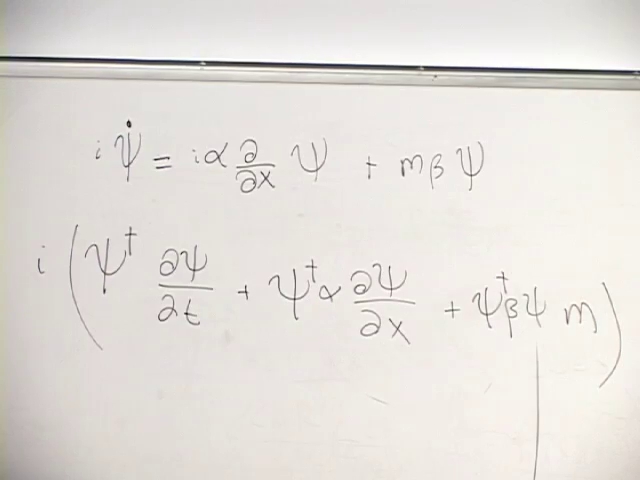
\includegraphics[width=0.76\textwidth]{lecture_09_figure_05.png}
\caption{حدود المشتقة الزمنية والمشتقة المكانية والكتلة في مناقشة حقل ديراك.}
\lectureframe{00:25:37}
\end{figure}

\begin{classroomqa}
\lecturetimestamp{00:26:37}
\audiencequestion{هل وُضع القوس في لاغرانجية ديراك المقترَحة في موضعه الصحيح، بحيث يضرب \(i\) التعبير بأكمله؟}
\lecturerresponse{لا يُبتّ هنا في هذا الموضع بثقة، وليس ذلك لازمًا للنقطة البنيوية: توجد لاغرانجية تولِّد معادلة ديراك.}
\end{classroomqa}

أضِف الآن مجالًا قياسيًا \(\phi\). إن الجداء الساذج \(\Psi^\dagger\Psi\,\phi\) ليس قياسيًا لورنتزيًا. وإدخال مصفوفة ديراك نفسها التي تظهر في حد الكتلة يعطي
\begin{equation}
\mathcal L_{\mathrm{int}}
\propto
\Psi^\dagger\beta\Psi\,\phi.
\end{equation}
وبصورة مكافئة، فإن \(\Psi^\dagger\beta\Psi\) هو الثنائي الخطي الديراكي القياسي. وعند مغايرة اللاغرانجية الكاملة يُضاف حد متناسب مع \(\phi\) إلى معادلة ديراك، ويُضاف مصدر متناسب مع \(\Psi^\dagger\beta\Psi\) إلى معادلة المجال القياسي. ويشتت كلٌّ من المجالين الآخر.

\begin{classroomqa}
\lecturetimestamp{00:28:03}
\audiencequestion{هل إن \(\beta\) المُدخلة في تآثر القياسي--الفرميوني هي \(\beta\) نفسها التي تظهر في حد كتلة ديراك؟}
\lecturerresponse{نعم. إنها مصفوفة ديراك نفسها.}
\end{classroomqa}

إن المقارنة
\begin{equation}
m\Psi^\dagger\beta\Psi
\qquad\hbox{and}\qquad
\Psi^\dagger\beta\Psi\,\phi
\end{equation}
تجعل الاقتران يبدو كما لو أنه معلمة كتلة استُبدلت بمجال قياسي. وسيعود هذا الملحظ عندما يُنظر قرب النهاية في مجال ذي قيمة فراغية غير صفرية.

حتى الآن كان التفسير كلاسيكيًا: تشتت الحزم الموجية حزمًا موجية أخرى. ولهذا الجبر نفسه معنى جسيمي أوضح حين تصبح الحقول مؤثرات.

\section{ما الذي تفعله أُسُس الحقول الكمومية}

يحتوي المجال الكمومي القياسي الحقيقي على مؤثرات الإنشاء والإفناء معًا. وعلى نحو تخطيطي،
\begin{equation}
\phi(x)\sim A^+(x)+A^-(x),
\end{equation}
حيث إن \(A^+\) ينشئ كمًّا و\(A^-\) يفني كمًّا. وعليه، يحتوي \(\phi^3(x)\) على أربعة أنواع من العمليات الموضعية:
\begin{equation}
\phi^3
\sim
(A^+)^3+(A^+)^2A^-+A^+(A^-)^2+(A^-)^3,
\end{equation}
حيث أُهملت في هذه القراءة التخطيطية تفاصيل الترتيب والمعاملات العددية. والتغيّرات الأربعة في عدد الجسيمات هي
\begin{equation}
3\longrightarrow0,
\qquad
0\longrightarrow3,
\qquad
2\longrightarrow1,
\qquad
1\longrightarrow2.
\end{equation}
وتؤثر عوامل المجال الثلاثة جميعًا في النقطة نفسها \(x\). ولذلك فإن حدًا تكعيبيًا واحدًا يضم إفناء ثلاثة جسيمات، وإنشاء ثلاثة جسيمات، واندماج كمّين في كمّ واحد، وانقسام كمّ واحد إلى كمّين. وفي سعة فيزيائية قد يُستبعد بعض هذه القراءات الموضعية لاحقًا بفعل حفظ الطاقة--الزخم، لكنها كلها موجودة في جداء المؤثرات نفسه.

للحدود الحرة التربيعية دور مختلف. أولًا، لِنُهمِل عامل تطبيع الفرق بين النقطتين المتجاورتين \(x\) و\(x'\):
\begin{equation}
\partial_x\phi
\ \propto\
\phi(x)-\phi(x').
\end{equation}
ويعطي التربيع والتوسيع بنية الحدود
\begin{align}
\frac12(\partial_x\phi)^2
&\ \propto\
\frac12\bigl[\phi(x)-\phi(x')\bigr]^2
\\
&=
\frac12\phi(x)^2
+\frac12\phi(x')^2
-\phi(x)\phi(x').
\end{align}
ولكل مربع عند النقطة نفسها عدة قراءات على مستوى المؤثرات: فقد ينشئ كمّين، أو يفني كمّين، أو يفني كمًّا ويعيد إنشاءه في تلك النقطة نفسها. وهذه الحدود لا تنقل جسيمًا. ويمكن للحد المتقاطع أن يفني كمًّا عند \(x'\) ويُنشئه عند \(x\)، أو بالعكس. ولذلك فهو يعمل حدَّ قفز بين أقرب الجيران. وتنقل العوامل المتكررة جسيمًا من \(x\) إلى \(x'\)، ثم إلى \(x''\)، وهكذا. وتحكم حدود المشتقة التربيعية الانتشار الحر؛ أما الحدود التكعيبية وما فوقها فتشتت الجسيمات وتُنشئها وتفنيها.

\begin{classroomqa}
\lecturetimestamp{00:36:07}
\audiencequestion{هل ينبغي أن يتضمن تمثيل المشتقة بالفروق المنتهية الفاصل \(x-x'\)؟}
\lecturerresponse{نعم. إذا سُمِّي هذا الفاصل \(L\) ظهر العامل \(L^{-2}\) بعد تربيع الفرق. وهذا العامل العددي يغيّر المعامل، لا تفسير القفز.}
\end{classroomqa}

وتعطي استعادة الفاصل
\begin{align}
\frac12(\partial_x\phi)^2
&\longrightarrow
\frac{1}{2L^2}\bigl[\phi(x)-\phi(x')\bigr]^2
\\
&=
\frac{1}{2L^2}\phi(x)^2
+\frac{1}{2L^2}\phi(x')^2
-\frac{1}{L^2}\phi(x)\phi(x').
\end{align}

حد الكتلة تربيعي أيضًا، لكنه لا يحتوي على مشتقة:
\begin{equation}
\frac12m^2\phi(x)^2.
\end{equation}
وقراءته أحادية الجسيم هي أن كمًّا واردًا يُمتص ثم يُعاد إصداره عند النقطة نفسها. وهو لا ينقل الكم؛ بل يزن وجوده هناك، أو بهذا المعنى يعدّه. ويحتوي مربع المؤثر نفسه أيضًا على قراءتي الإنشاء المزدوج والإفناء المزدوج. لذا فالتمييز المرتبط بالحركة هو بين حد تبادلي يصل بين نقطتين متجاورتين وإدراج كتلة يعمل داخل نقطة واحدة.

\section{الرأس الموضعي في الكهروديناميكا الكمية}

هذه الرسوم التخطيطية الأولية لعمليات الجسيمات هي بدايات مخططات فاينمان. والمثال المركزي هو الكهروديناميكا الكمية، وهي نظرية الإلكترونات والبوزيترونات والفوتونات.

لمعادلة ديراك أنماط ذات طاقة موجبة وأخرى ذات طاقة سالبة. وفي الاصطلاح الأقدم، يحتوي \(\Psi\) على مؤثرات إفناء لكلا نوعي الأنماط، بينما يحتوي \(\Psi^\dagger\) على مؤثرات الإنشاء المناظرة. وتُعادُ إعادةُ تفسير إزالة إلكترون ذي طاقة سالبة على أنها إنشاء بوزيترون ذي طاقة موجبة. وبعد إعادة التسمية هذه، يكون التحليل التخطيطي المفيد هو
\begin{align}
\Psi
&\sim
C^-_{e^-}+C^+_{e^+},
\\
\Psi^\dagger
&\sim
C^+_{e^-}+C^-_{e^+}.
\end{align}
وهكذا فإن \(\Psi\) يفني إلكترونًا أو ينشئ بوزيترونًا، بينما ينشئ \(\Psi^\dagger\) إلكترونًا أو يفني بوزيترونًا. ولا يُقصد بهذا الاختصار أي عامل تطبيع أو مؤشر لف مغزلي أو تكامل على الزخم.

يقترن تآثر الكهروديناميكا الكمية بتيار ديراك مع الكمون المتجهي الكهرومغناطيسي. وفي ترميز المركبات المستعمل هنا، تكون بنيته
\begin{equation}
\mathcal L_{\mathrm{QED,int}}
\sim
e\left(
\Psi^\dagger\Psi\,A_0
+
\Psi^\dagger\boldsymbol{\alpha}\Psi\mathbin{\boldsymbol{\cdot}}\mathbf A
\right),
\end{equation}
حيث
\begin{equation}
J^0=\Psi^\dagger\Psi,
\qquad
\mathbf J=\Psi^\dagger\boldsymbol{\alpha}\Psi.
\end{equation}
والرمز \(\sim\) مهم: فالإشارة النسبية بين الحدين الزمني والمكاني تعتمد على اصطلاحي المتريّة والكمون المتجهي. أما العبارة الثابتة فهي أن التيار الرباعي يُعقَد مع الكمون الرباعي.\editorialnote{يحدد المصدر المركبتين الزمنية والمكانية للتيار، لكنه لا يحسم اصطلاحًا للمتريّة في عقد المركبات.}

يحتوي حقل الفوتون \(A_\mu\) نفسه على مؤثرات إنشاء الفوتونات وإفنائها. كما أن طبيعته المتجهية تحمل أيضًا استقطاب الفوتون---أي ``علامة'' اتجاهية صغيرة بالإضافة إلى زخمه.

\begin{classroomqa}
\lecturetimestamp{00:44:28}
\audiencequestion{كيف يمكن أن يكون التآثر قياسيًا بينما يكون \(A_\mu\) متجهًا ويبدو عامل الفرميون في البداية كمية قياسية؟}
\lecturerresponse{توفر الفرميونات أيضًا متجهًا رباعيًا: \(\Psi^\dagger\Psi\) هو مركبته الزمنية و\(\Psi^\dagger\boldsymbol\alpha\Psi\) مركبته المكانية. وعقد ذلك التيار مع \(A_\mu\) ينتج كمية قياسية.}
\end{classroomqa}

بضرب المحتوى المؤثري لـ \(\Psi^\dagger\) و\(\Psi\) و\(A_\mu\) نحصل على أربعة تفسيرات مألوفة لرأس موضعي واحد:
\begin{enumerate}
\item يصدر إلكترون فوتونًا؛
\item يمتص إلكترون فوتونًا؛
\item يفنى إلكترون وبوزيترون في فوتون؛
\item يُنشئ فوتون زوج إلكترون--بوزيترون.
\end{enumerate}
في التفسير الأول، يفني \(\Psi\) الإلكترون الوارد، وينشئ \(\Psi^\dagger\) الإلكترون الصادر، وينشئ حقل الفوتون الفوتون. واختيار جزء إفناء الفوتون يعطي الامتصاص. واختيار الأجزاء الخاصة بالبوزيترون يعطي فناء الزوج أو إنشاء الزوج. ويحتوي حد موضعي واحد العائلة كلها.

في مخطط تدفق الفرميونات، يشير السهم على خط البوزيترون عكس اتجاه انتشار البوزيترون. وبهذا الاصطلاح يمر سهم الفرميون بلا انقطاع عبر كل رأس مسموح به في الكهروديناميكا الكمية. وتختلف التفسيرات الأربعة بنقل الأرجل الخارجية بين جانبي الوارد والصادر، لا بكسر خط تدفق الفرميون.

كل واحد من هذه التفسيرات يحمل المعامل نفسه \(e\)، وهو الشحنة الكهربائية في الاصطلاح المجهري المستعمل. وهذا المعامل هو الشحنة الكهربائية \(e\)، وليس ثابت البنية الدقيقة، مع أن كليهما مرتبط بالآخر ارتباطًا وثيقًا. وسعة الرأس تتناسب مع \(e\)؛ وبعد إدراج جميع العوامل الحركية وعوامل التطبيع، يتناسب مقياس الاحتمال الموافق مع \(e^2\).

\begin{classroomqa}
\lecturetimestamp{00:49:44}
\audiencequestion{هل لتفسير فوتون إلى إلكترون--بوزيترون المعامل نفسه مثل سائر تفسيرات الرأس؟}
\lecturerresponse{نعم. فهو يحمل معامل الشحنة الكهربائية نفسه \(e\).}
\end{classroomqa}

\begin{classroomqa}
\lecturetimestamp{00:49:59}
\audiencequestion{هل لا بد من وجود عامل تحجيم، بما أن الاحتمال لا وحدة له؟}
\lecturerresponse{في الاصطلاح المجهري الطبيعي المستخدم هنا، تكون الشحنة \(e\) عديمة الأبعاد. فهي مقياس السعة، بينما يمد مربعها بمقياس الاحتمال.}
\end{classroomqa}

وصورة ملموسة لذلك هي إلكترون يصطدم بجدار ويتوقف فجأة. وهناك بعض الاحتمال لأن تغادر الطاقة والزخم على هيئة فوتون. والعامل الكهرومغناطيسي الأولي في سعة هذا الإشعاع هو \(e\)، لذا فإن مقياس احتماله يحتوي على \(e^2\). وهذه العبارة تعزل عامل الاقتران؛ فالاحتمال الفعلي يعتمد أيضًا على حالة الإلكترون وعلى الحركيات.

\begin{figure}[htbp]
\centering
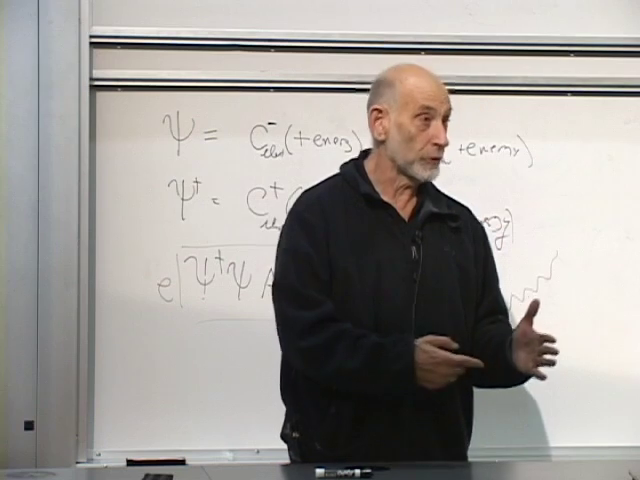
\includegraphics[width=0.78\textwidth]{lecture_09_figure_06.png}
\caption{محتوى مؤثرات الإلكترون والبوزيترون في \(\Psi\) و\(\Psi^\dagger\)، مع رسم تخطيطي لتآثر إلكترون--فوتون.}
\lectureframe{00:50:39}
\end{figure}

\begin{classroomqa}
\lecturetimestamp{00:51:15}
\audiencequestion{هل للشحنة الكهربائية وحدات؟}
\lecturerresponse{ليس في الاصطلاح المجهري الطبيعي المستخدم هنا. فكثيرًا ما تُعطى الشحنة العيانية بالكولوم، لكن نظرية الجسيمات تقيس الشحنة نسبةً إلى وحدة أولية مختارة. وفي وحدات بلانك أو غيرها من الوحدات الطبيعية تُعبَّر الكميات على هيئة أعداد محضة.}
\end{classroomqa}

يكمن التباين في الاصطلاحات والمقاييس. فالكولوم ملائم للتيار في الأسلاك؛ والاقتران العديم الأبعاد ملائم للسعات المجهرية.\editorialnote{سؤال موجز من 00:52:37--00:53:15 حول ``تجميع'' الحدود الحاملة للشحنة تالف إلى حد كبير، ولم يفض إلى صياغة محددة.}

تُقيَّم الحقول الثلاثة جميعًا في التآثر الأولي للكهروديناميكا الكمية عند نقطة واحدة في الزمكان. ولا يُسنَد إلى الرأس نفسه أي تأخر زمني داخلي.

\begin{classroomqa}
\lecturetimestamp{00:53:19}
\audiencequestion{هل يكون امتصاص الإلكترون وإعادة إصداره وانبعاث الفوتون متزامنة، أم أن المعادلة تُضمّن تأخرًا؟}
\lecturerresponse{في الرأس الأولي تُقيَّم جميع المؤثرات عند النقطة نفسها من الزمكان. لذلك لا تتضمن العملية الأساسية أي تأخر بين تلك الأفعال.}
\end{classroomqa}

\begin{classroomqa}
\lecturetimestamp{00:53:57}
\audiencequestion{هل يجب أن تُحفظ كل كمية محفوظة على حدة؟}
\lecturerresponse{نعم. والشحنة الكهربائية إحدى الكميات التي يجب أن تُحفظ على حدة.}
\end{classroomqa}

يظهر حفظ الشحنة في كل من المخطط والجبر. فالعملية التي تحوِّل إلكترونًا واردًا إلى بوزيترون صادر تقلب الشحنة، وليست رأسًا مسموحًا به في الكهروديناميكا الكمية. وعندما يُرسم الزمن إلى الأعلى، يتبع سهم الإلكترون اتجاه الزمن إلى الأعلى ويشير سهم البوزيترون إلى الأسفل؛ ويكون في الرأس الصحيح دائمًا سهم فرميوني يمر عبره. جبريًا، يحتوي التآثر على \(\Psi\) واحد و\(\Psi^\dagger\) واحد. فالأول يرفع الشحنة بمقدار وحدة واحدة عندما يفني إلكترونًا أو ينشئ بوزيترونًا، والثاني يخفضها بمقدار وحدة واحدة. وتتلاشى آثارهما.

\begin{classroomqa}
\lecturetimestamp{00:56:05}
\audiencequestion{هل التعبير المؤطر للإلكترون--الفوتون هو لاغرانجيان الكهروديناميكا الكمية كله؟}
\lecturerresponse{لا. إنه حد التآثر. ولم تُكتب الحدود الحرة التربيعية للفوتون ولا حدود ديراك التربيعية التي تحكم الانتشار.}
\end{classroomqa}

\begin{classroomqa}
\lecturetimestamp{00:56:35}
\audiencequestion{هل يُستنتج لاغرانجيان كلاسيكي بينما يُخمَّن لاغرانجيان كمي ويُختبر، وهل تبقى بنية الحركية ناقص الجهد في ميكانيكا الكم؟}
\lecturerresponse{يبقى نمط الحركية ناقص الجهد: فمشتقات الزمن تعطي الصورة الحركية، وتعممها التدرجات المكانية، وتعطي حدود الحقول غير المشتقة الصورة الجهدية. ولاغرانجيان الكمي هو الوصف الأكثر أساسية. وفي حالة تحتوي عددًا كبيرًا جدًا من الكمات، ينتج لاغرانجيان نفسه معادلات الموجات الكلاسيكية. وتُقترح اللاغرانجيانات المرشحة باستخدام المبادئ الفيزيائية ونظرية أعمق، ثم تُثبَت أو تُرفَض عبر تجارب التصادم.}
\end{classroomqa}

يفسر حد الإشغال الكبير لماذا يمكن للتعبير نفسه أن يحكم نظرية جسيمات كمية وموجاتها الكلاسيكية. وهذا التوافق ليس معجزة مستقلة فُرضت بعد ذلك؛ فالحقل الكلاسيكي هو السلوك الجمعي لعدد كبير من الكمات. وعلى العكس من ذلك، تكشف التصادمات التجريبية الرؤوس الأولية مباشرةً بما يكفي لتحديد تآثرات الكهروديناميكا الكمية والنموذج المعياري بدقة كبيرة.

\section{العبور وقوانين الحفظ في الزمكان}

يمكن تبديل أرجل رأس موضعي بين موضعي الداخل والخارج. فالجسيم الخارج الذي يُنقل إلى جهة الداخل يُعاد تفسيره على أنه جسيمه المضاد، وبالعكس. وبهذا المعنى فإن مؤثر الإلكترون--البوزيترون--الفوتون نفسه له قراءة موضعية على أنها انبعاث، وامتصاص، وفناء زوجي، وخلق زوجي، وحتى قراءة يكون فيها الجميع داخلين.

\begin{classroomqa}
\lecturetimestamp{00:59:34}
\audiencequestion{إذا أُدير مخطط رأس أساسي، فهل يظل قراءة موضعية صحيحة؟}
\lecturerresponse{نعم. يمكن نقل أرجله الخارجية بين موضعي الداخل والخارج، مع إعادة التفسير المناظرة للجسيم--الجسيم المضاد.}
\end{classroomqa}

القراءة المؤثرية الموضعية ليست بعدُ عملية فيزيائية مكتملة. ويجب تكامل سعتها على كل نقطة في الزمكان يمكن أن يحدث عندها الرأس. فتكامل الزمن يفرض حفظ الطاقة، وتكامل المكان يفرض حفظ الزخم. والصورة التي يختفي فيها إلكترون وبوزيترون وفوتون جميعًا في الفراغ موجودة بوصفها قراءة موضعية صورية، لكن السعة المتكاملة تنعدم لأن العملية لا يمكنها أن تحفظ الطاقة والزخم.

\begin{classroomqa}
\lecturetimestamp{01:00:30}
\audiencequestion{هل تعني الصورة التي يكون فيها الجميع داخلين أن إلكترونًا وبوزيترونًا وفوتونًا يمكن أن يختفوا في العدم؟}
\lecturerresponse{إنها قراءة للمؤثر الموضعي، لكن السعة الفيزيائية تتضمن تكاملًا على موضع الرأس. وتفرض تلك التكاملات حفظ الطاقة والزخم، لذا فهذه العملية الممنوعة حركيًا سعتها صفر.}
\end{classroomqa}

\begin{classroomqa}
\lecturetimestamp{01:01:57}
\audiencequestion{وهل توجد أيضًا القراءة العكسية من الفراغ إلى إلكترون--بوزيترون--فوتون، وهل تختفي العمليات المستبعَدة بعد التكامل؟}
\lecturerresponse{القراءة الموضعية العكسية موجودة أيضًا. والتكامل على المكان والزمان يزيل أي عملية لا تنسجم مع قوانين الحفظ.}
\end{classroomqa}

تنسجم المشتقات في اللاغرانجيان مع التوسع المؤثري من غير أن يُشتق رمزا الخلق والفناء نفسيهما. وللحقل الصورة التخطيطية
\begin{equation}
\Psi(x)
\sim
\int d^3k\,
\bigl[
C(\mathbf k)e^{i\mathbf k\cdot\mathbf x-i\omega t}
+\cdots
\bigr].
\end{equation}
والمؤثرات \(C(\mathbf k)\) هي معاملات في هذا التوسع الزمكاني. وتؤثر المشتقات في الموجات المستوية فتُنزل \(\mathbf k\) أو \(\omega\).

\begin{classroomqa}
\lecturetimestamp{01:02:27}
\audiencequestion{عند اشتقاق توسع حقل، هل يُشتق مؤثر الخلق نفسه؟}
\lecturerresponse{لا. مؤثرا الخلق والفناء مستقلان عن إحداثي الزمكان في هذا التوسع. وتؤثر المشتقات في العوامل الأسية وتُنزل الزخم والتردد.}
\end{classroomqa}

\section{النيوكليونات والبيونات بوصفها نظرية فعالة}

يمكن للغة نفسها أن تصف البروتونات والنيوترونات والبيونات. فالبروتونات والنيوترونات فرميونات تمثلها الحقول \(\Psi_p\) و\(\Psi_n\). وفي هذا النقاش الخاص بعدّ التفاعلات، تُعامَل حقول البيون على أنها حقول قياسية بثلاثة أصناف من الشحنة،
\begin{equation}
\pi^+,
\qquad
\pi^-,
\qquad
\pi^0.
\end{equation}
يحمل البروتون و\(\pi^+\) وحدة موجبة واحدة من الشحنة الكهربائية، ويحمل \(\pi^-\) وحدة سالبة واحدة، أما النيوترون و\(\pi^0\) فمتعادلَان. وعلى مستوى أعمق، البيونات منظومات كوارك--ضديد كوارك، لكن يمكن في البداية ترك هذا الوصف الداخلي دون حسم.

قائمة تخطيطية محافظة على الشحنة لجداءات حقول النيوكليون--البيون هي
\begin{equation}
\mathcal L_{N\pi}
\sim
\left\{
\Psi_p^\dagger\Psi_n\,\pi^+,\;
\Psi_n^\dagger\Psi_p\,\pi^-,\;
\Psi_p^\dagger\Psi_p\,\pi^0,\;
\Psi_n^\dagger\Psi_n\,\pi^0
\right\}.
\end{equation}
المعروض هنا هو فقط محتوى الحقول وإسنادات الشحنة؛ أما المعاملات النسبية، والإشارات، وبنية المصفوفة السبينورية، فلا تُثبَّت هنا. وتتحدد شحنة حقل البيون الأول باختبار قراءة محددة: فبإمكان نيوترون مع بيون موجب أن ينتجا بروتونًا، بينما استعمال بيون سالب هناك من شأنه أن يحول شحنة داخلة سالبة إلى شحنة خارجة موجبة. ويعطي الحد المرافق العملية ذات الشحنة المعاكسة.\editorialnote{صُحِّحت إشارة البيون عدة مرات في المصدر قبل الوصول إلى الزوج المحافظ على الشحنة المعروض هنا؛ والترتيب المعروض يسجل تلك البنية التخطيطية النهائية.}

ولكل حد مرة أخرى عدة قراءات متقاطعة. فنقل نيوترون خارج إلى جهة الداخل يحوله إلى ضديد نيوترون داخل. ولذلك يمكن للرأس المشحون أن يصف بروتونًا وضديد نيوترون يتحدان في \(\pi^+\)، وكذلك عمليات مثل \(p\to n+\pi^+\) عندما تسمح الحركيات بذلك. وتتيح الحدود المتعادلة لبروتون أو نيوترون أن يصدر أو يمتص \(\pi^0\). ويختار حفظ الشحنة العائلة المسموح بها، بينما تحدد الطاقة والزخم وأي تناظرات إضافية أيَّ فرد منها يمكن أن يقع في تجربة معينة.

كان هذا وصفًا فعالًا مفيدًا قبل أن تُعرف البنية التحتية الكواركية. وما يزال مفيدًا كلما عجز المسبار عن تمييز تلك البنية. فللبروتون توزع متناهٍ في الامتداد لمكوناته، على نحو يشبه امتلاك الذرة بنية داخلية، وإن كان على مقياس أصغر بكثير. وإذا نقلت تجربة زخمًا قليلًا جدًا بحيث لا يكفي لتفكيك البروتون أو تمييزه، أمكن معاملة البروتون بوصفه جسيمًا نقطيًا له حقله الخاص. أما التصادم الشديد بما يكفي فيكشف الكواركات، وعندئذٍ لا يعود حقل البروتون الجسيمي النقطي كافيًا.

ولأن البروتون مشحون، فله أيضًا تآثر موضعي بروتون--فوتون، تخطيطيًا \(J_p^\mu A_\mu\)، حيث إن \(J_p^\mu\) هو تيار البروتون. وللإلكترون تآثره المناظر إلكترون--فوتون. ولا يمكن للبروتون بدلًا من ذلك أن يتحول إلى نيوترون بإصدار فوتون: إذ إن \(p\to n+\gamma\) ينتهك حفظ الشحنة.

\begin{classroomqa}
\lecturetimestamp{01:10:28}
\audiencequestion{ماذا يحدث عندما يتآثر بروتون وإلكترون؟}
\lecturerresponse{لكل جسيم مشحون رأس فوتون. يمكن للبروتون أن يصدر فوتونًا مع بقائه بروتونًا، ويمكن للإلكترون أن يمتص الفوتون مع بقائه إلكترونًا. ويُبنى تشتت البروتون--الإلكترون من هذين الرأسين الموضعيين وانتشار الفوتون بينهما.}
\end{classroomqa}

\section{الموضعية والعمليات الأولية المتكررة}

لا يوجد حد لا موضعي خاص للتبادل الكامل بروتون--إلكترون. فرأس موضعي واحد يصدر الفوتون عند البروتون، وتنقله الحدود التربيعية للفوتون من نقطة مجاورة إلى نقطة مجاورة، ويمتصه رأس موضعي آخر عند الإلكترون. والعملية الممتدة هي حاصل ضرب تلك القطع الأولية.
\begin{equation}
\begin{aligned}
\bigl[J_p^\mu A_\mu\bigr](x_p)
&\longrightarrow
\underbrace{x_p\to x_1\to x_2\to\cdots\to x_e}_{\text{quadratic photon propagation}}
\\
&\longrightarrow
\bigl[J_e^\nu A_\nu\bigr](x_e).
\end{aligned}
\end{equation}
والأسهم في هذه السلسلة التخطيطية تدل على إدخالات متعاقبة بين نقاط متجاورة، لا على تآثر لا موضعي جديد.

\begin{classroomqa}
\lecturetimestamp{01:12:06}
\audiencequestion{كيف يكتب المرء اللاغرانجيان للتبادل الكامل بروتون--إلكترون؟}
\lecturerresponse{لا يضاف حد للحدث الممتد كله. بل يُبنى من رأس موضعي بروتون--فوتون، وحدود انتشار تربيعية متكررة، ورأس موضعي إلكترون--فوتون.}
\end{classroomqa}

للبنية الموضعية صورتان. فحد التآثر غير المشتق يؤثر عند نقطة واحدة في الزمكان. أما الحد المشتق، المعبَّر عنه بفارق منتهٍ، فيصل تلك النقطة بنقطة مجاورة فقط. ولا ينقل أي من النوعين جسيمًا مباشرة عبر مسافة منتهية. فالانتشار بعيد المدى يُركَّب من انتقالات متناهية الصغر كثيرة؛ ولا يوجد تأثير أولي عن بُعد.

\begin{classroomqa}
\lecturetimestamp{01:14:36}
\audiencequestion{هل يحتوي اللاغرانجيان على حدود عند نقطة واحدة فقط؟}
\lecturerresponse{تؤثر حدود التآثر عند نقطة واحدة. أما الحدود المشتقة فتصل نقطة بنقطة مجاورة لها على نحو متناهٍ في القرب. ويؤدي الإصدار، ثم القفزات الكثيرة بين النقاط المتجاورة، ثم الامتصاص معًا إلى تبادل منتهٍ.}
\end{classroomqa}

\begin{classroomqa}
\lecturetimestamp{01:15:36}
\audiencequestion{هل جميع قطع العملية الممتدة موجودة، وهل يعني تركيبها أخذ حاصل ضربها؟}
\lecturerresponse{نعم. فكل إصدار أولي، أو قفزة، أو امتصاص، مُرمَّز له في اللاغرانجيان. وتُركِّب جداءات الإدخالات المتكررة تلك القطع في العملية الأكبر.}
\end{classroomqa}

تفترض نظرية الحقل الكمومي النسبية قيد المناقشة الإطار الزمكاني الذي تُعرَّف عليه حقولها. ولا ينبغي الخلط بينها وبين نظرية كمومية كاملة لهندسة زمكانية ديناميكية.

\begin{classroomqa}
\lecturetimestamp{01:16:28}
\audiencequestion{هل يظل هذا التركيب صالحًا في وضع نسبي شديد، مثل القرب من أفق ثقب أسود؟}
\lecturerresponse{امتداد ذلك إلى حالة الثقب الأسود خارج نطاق هذا البناء. فنظرية الحقل الكمومي المستعملة هنا لا توفر بذاتها وصفًا كاملًا لديناميكيات الثقوب السوداء، حيث تكون الجاذبية أساسية.}
\end{classroomqa}

الحقل مؤثر لفعل موضعي أولي. ويمكن لعامل حقلي واحد أن يمتص جسيمًا أو أن يصدر جسيمًا. ويمكن لجداء عاملين أن يمتص جسيمًا ويصدر آخر عند النقطة نفسها؛ كما تستطيع الجداءات الأعلى رتبة أن تغير محتوى الجسيمات أكثر. وتصل جداءات المؤثرات الموضعية هذه الأفعال في تواريخ. وفي الزمكان تُمثَّل الحركة بامتصاص في منطقة صغيرة، ثم إعادة إصدار إلى منطقة مجاورة، ثم امتصاص آخر، ثم إعادة إصدار أخرى. وجعل طول الخطوة يقترب من الصفر مع ازدياد عدد الخطوات يعطي المسار المتصل.

\begin{classroomqa}
\lecturetimestamp{01:17:30}
\audiencequestion{كيف ينبغي فهم الحقول والمسافة والزمن في هذه الصورة القائمة على الخطوات المحلية؟}
\lecturerresponse{الحقول هي مؤثرات للامتصاص والإصدار المحليين. وتربط المضروبات بين تلك الأفعال الأولية، وتُبنى الحركة عبر الزمكان من خطوات متناهية الصغر بين المواضع المتجاورة قبل أخذ حد المتصل.}
\end{classroomqa}

ولذلك فإن نقطة بداية منظَّمة هي تقسيم الزمكان إلى خلايا صغيرة، مع إلحاق مؤثرات الحقل بالخلايا.\editorialnote{صياغة الحضور عند 01:17:30--01:20:40 محجوبة جزئياً؛ والسؤال المعاد بصياغته لا يحتفظ إلا بموضوعه الذي أمكن استرجاعه، بينما الجواب عن المؤثرات المحلية وخطوات الزمكان المتعاقبة واضح.} وتتحول المشتقات إلى فروق. وتصل الحدود التربيعية المختلطة بين الخلايا المتجاورة، بينما تؤثر حدود الكتلة والتفاعل داخل خلية واحدة. والخلايا أداة لتعريف النظرية الحدية، وليست جسيمات إضافية ولا مقياساً فيزيائياً جديداً للكتلة.

لا يلزم أن تُضاف تأثيرات النسبية الخاصة على نحو منفصل في كل خطوة. فإذا كان اللاجرانجي كمية قياسية لورنتزية، فإن السعات المجمَّعة منه تكون ثابتة تحت تحولات لورنتز، وتترتب تأثيرات مثل تمدد الزمن على تلك البنية.

\begin{classroomqa}
\lecturetimestamp{01:21:10}
\audiencequestion{هل تخلق الحركة عالية الطاقة وتمدد الزمن مشكلات إضافية في عملية متعددة الخطوات؟}
\lecturerresponse{لا يلزم تصحيح منفصل. فإذا كان اللاجرانجي كمية قياسية لورنتزية، فإن تأثيرات النسبية الخاصة مثل تمدد الزمن مدمجة بالفعل في النتيجة. أما منشأ القلق المحدد الكامن وراء السؤال فليس واضحاً تماماً.}
\end{classroomqa}

يمكن تمثيل مؤثرات الإنشاء والإفناء في أساس الموضع أو في أساس الزخم. ومؤثر الإنشاء في فضاء الموضع هو تراكب فورييه لمؤثرات الإنشاء في فضاء الزخم، وبالعكس. ولا يوجد مؤثر ينشئ حالة يكون فيها الموضع محدداً بدقة والزخم محدداً بدقة في آن واحد. فتوطين الجسيم على نحو حاد يتطلب نطاقاً واسعاً من الزخوم؛ وتوطينه على نحو حاد في الزخم ينشره على الموضع. وعلاقة فورييه بين الأساسين هي مبدأ عدم اليقين بهذه اللغة.

\begin{classroomqa}
\lecturetimestamp{01:22:48}
\audiencequestion{كيف ترتبط مؤثرات الإنشاء والإفناء بالموضع والزخم ومبدأ عدم اليقين؟}
\lecturerresponse{يمكن تمثيلها بوصفها توابع للموضع أو توابع للزخم. والتمثيلان تحويل فورييه أحدهما للآخر. فالحالة الحادة التوضع في الموضع تتطلب كثيراً من الزخوم، بينما تكون الحالة الحادة في الزخم ممتدة على الموضع؛ ولا يوجد مؤثر إنشاء لـ \(x\) و\(p\) محددين بحدة في آن واحد.}
\end{classroomqa}

يمكن الآن صياغة بناء الخلايا بالكامل. وسِم الخلايا بـ \(n\)، واستبدل المشتق بفارق منتهٍ مثل
\begin{equation}
\partial_\mu\phi(x)
\longrightarrow
\frac{\phi_{n+\hat\mu}-\phi_n}{a},
\end{equation}
وضع كل نوع حقلي في كل خلية. حد تربيعي مختلط يزيل كمّاً من خلية ويُنشئه في خلية مجاورة. وتُستعاد نظرية المتصل بأخذ التباعد \(a\) نحو الصفر بعد تعريف التعابير المنظَّمة.
\begin{equation}
\underbrace{\phi_n\phi_{n+\hat\mu}}_{\text{hop }n\leftrightarrow n+\hat\mu},
\qquad
\underbrace{m^2\phi_n^2}_{\text{same-cell mass insertion}}.
\end{equation}

\begin{classroomqa}
\lecturetimestamp{01:25:16}
\audiencequestion{هل يمكن إتمام تقسيم الزمكان إلى خلايا؟}
\lecturerresponse{نعم. تُفهرس الحقول بالخلايا، وتتحول المشتقات إلى فروق منتهية، وتنقل الحدود التربيعية الجسيمات قفزاً بين الخلايا المتجاورة. ويُستعاد المتصل عندما يؤول حجم الخلية إلى الصفر.}
\end{classroomqa}

تقفز الإلكترونات بين الخلايا عبر حدودها التربيعية، وكذلك تفعل الفوتونات. وعندما يجتمع إلكترون وفوتون في خلية واحدة، يمكن لتفاعل QED أن يمتص الإلكترون ويعيد إصداره مع إنشاء الفوتون أو إفنائه. ولحد الكتلة القياسي قراءة داخل الخلية نفسها: يدخل الجسيم تلك الخلية ويغادرها بمعامل يتناسب مع \(m^2\). وهو لا يوفّر قفزة.

\begin{classroomqa}
\lecturetimestamp{01:28:18}
\audiencequestion{هل يرتبط حجم الخلية بمعامل الكتلة؟}
\lecturerresponse{لا. حجم الخلية هو تباعد تنظيمي يُؤخذ في النهاية إلى الصفر؛ أما معامل الكتلة فهو وسيط مستقل في اللاجرانجي.}
\end{classroomqa}

\begin{classroomqa}
\lecturetimestamp{01:28:43}
\audiencequestion{هل ضرب العوامل المحلية هو بناء لسعة مشتركة على امتداد الزمكان، لا مجرد تعاقب زمني؟}
\lecturerresponse{نعم. تغطي الخلايا الزمكان، وتتجمع إسهاماتها المحلية عبر شبكة الزمكان تلك. ويعطي المضروب سعة مشتركة للأحداث المحلية المطلوبة وخطوات الانتشار.}
\end{classroomqa}

\section{المصادر والكواشف والديناميات بينهما}

العملية الكاملة هي تاريخ في الزمكان. ويتحدد شرطها الابتدائي بما يهيئه المجرِّب، وشرطها النهائي بما تسجله الكواشف. ومصدر بسيط هو فتيلة ساخنة تبعث إلكتروناً. فمؤثر حقلي عند الفتيلة ينشئ ذلك الإلكترون الوارد؛ ومؤثرات حقلية عند مواضع الكواشف تصف امتصاصه في نهاية المطاف.

\begin{classroomqa}
\lecturetimestamp{01:29:30}
\audiencequestion{ما المرحلة الابتدائية لمثل هذه العملية في الزمكان؟}
\lecturerresponse{تُهيَّأ عند المصادر. والإلكترون المنبعث من فتيلة ساخنة مثال بسيط: فمؤثر حقلي عند الفتيلة ينشئ الإلكترون، بينما تحدد مؤثرات حقلية عند الكواشف أحداث الامتصاص النهائية.}
\end{classroomqa}

يمكن كذلك صياغة البناء نفسه انطلاقاً من الخلاء. فمؤثرات الإنشاء عند المصادر تبني الحالة الداخلة على الخلاء. ومؤثرات الإفناء المرتبطة بالكواشف تنتقي الحالة الخارجة. وهذه المؤثرات تحدد الشروط الحدية؛ وهي لا تحل محل الديناميات في كامل المنطقة بين المصدر والكاشف.

\begin{classroomqa}
\lecturetimestamp{01:31:11}
\audiencequestion{هل يكون من الخطأ حصر الديناميات في البواعث وحدها بدلاً من امتدادها في النظام كله؟}
\lecturerresponse{نعم. ابدأ من الخلاء، واستعمل مؤثرات المصدر لتهيئة الجسيمات الداخلة، واستعمل مؤثرات الكاشف لانتقاء الجسيمات النهائية. وبينهما تعمل إدخالات اللاجرانجي المتكررة في الزمكان كله، فتنقل الجسيمات، وتنشئها، وتفنيها.}
\end{classroomqa}

ومع عدد كافٍ من الإدخالات، يمكن لعدة جسيمات أن تتحرك في آن واحد عبر كثير من الخلايا المتجاورة؛ كما يمكن إنشاء الجسيمات أو إفناؤها على طول الطريق. وتبيّن المؤثرات الابتدائية ما الذي يدخل، وتبيّن المؤثرات النهائية ما الذي يُسجَّل، وتوفر عمليات اللاجرانجي المتكررة كل ما بينهما.

\begin{classroomqa}
\lecturetimestamp{01:33:24}
\audiencequestion{إذا أمكن حدوث عدد اعتباطي من إدخالات اللاجرانجي، فهل يُكامل على مواضعها؟}
\lecturerresponse{نعم. يُكامل على مواضعها في الزمكان. ولا تُشتق قواعد فاينمان الدقيقة هنا؛ وإنما النقطة المباشرة هي أن تعابير حقلية محلية بسيطة ترمّز إلى التفاعلات الأولية التي تُركَّب منها عملية كاملة.}
\end{classroomqa}

\section{تناظر الطور والشحنة والسعات}

إن كتابة العمليات الأولية في اللاجرانجي تجعل تناظراتها مرئية أيضاً. اعتبر تحول طور شامل لحقل الإلكترون،
\begin{equation}
\Psi\longrightarrow e^{i\theta}\Psi,
\qquad
\Psi^\dagger\longrightarrow e^{-i\theta}\Psi^\dagger,
\qquad
A_\mu\longrightarrow A_\mu.
\end{equation}
فالحد الذي يحتوي على عدد متساوٍ من \(\Psi\) و\(\Psi^\dagger\) لا يتغير لأن الأطوار تتلاشى فيما بينها. أما الحد ذو العددين غير المتساويين فسيكتسب طوراً. وتساوي هذين العددين هو الصورة الجبرية لانحفاظ الشحنة.

وهذه ميزة مركزية للوصف باللاجرانجي. فعوامله الحقلية تُظهر العمليات الأولية، وتُظهر تراكيبها التناظرات، وتُظهر التناظرات قوانين الانحفاظ. وتحول الإدخالات المتكررة الحالة الابتدائية المهيأة إلى الحالة النهائية المنتقاة. والنتيجة هي سعة كمومية. ويتطلب التقييم الدقيق قواعد فاينمان، لكن المحتوى البنيوي ظاهر بالفعل: فالعمليات المحلية تتكرر بكل ترتيب تسمح به قوانين الانحفاظ.

\section{قياسات الحقول والمبدلات}

تحتفظ مؤثرات الحقل بالمعنى المعتاد للمؤثرات في ميكانيكا الكم. فقيمها الذاتية هي النتائج الممكنة لقياسات الحقل، ومتجهاتها الذاتية تصف الحالات المرتبطة بتلك القيم. ويمكن سبر مجال كهربائي بوضع جسيم مشحون فيه ومراقبة كيف يتسارع ذلك الجسيم.

\begin{classroomqa}
\lecturetimestamp{01:37:06}
\audiencequestion{هل تؤدي القيم الذاتية والمتجهات الذاتية لمؤثرات الحقل دورها المعتاد في ميكانيكا الكم؟}
\lecturerresponse{نعم. القيم الذاتية هي القيم الحقلية الممكنة في القياس، ويمكن سبر الحقول من خلال تأثيراتها في الجسيمات. وتحدد المبدلات القيود على القياسات المتزامنة.}
\end{classroomqa}

الهوية التافهة
\begin{equation}
[\phi(x),\phi(x)]=0
\end{equation}
لا تحسم مسألة القياس. فلا بد من تحديد مرصودين وعلاقتهما الزمكانية. ويشكّل الحقل وزخمه المرافق زوجًا قانونيًا لا يتبادل، ومؤثرات الحقل عند نقاط يفصل بينها فاصل زمني قد لا تتبادل؛ أما الحقول البوزونية المحلية عند فصل مكاني فتتبادل، كما تقتضيه المحلية. ومن ثم تنتقل العلاقة المألوفة بين المبدِّلات وعدم اليقين إلى هنا أيضًا، ولكن فقط بعد تعيين زوج المؤثرات تعيينًا صحيحًا.\editorialnote{يعرض المصدر عدمَ التبادل عند نقاط متميزة على نحو أوسع مما ينبغي. والتقييد الوارد هنا يحافظ على مغزاه المتعلق بالقياس مع فرض السببية الميكروية للحقول البوزونية المحلية ذات الفصل المكاني.}

\begin{classroomqa}
\lecturetimestamp{01:39:57}
\audiencequestion{هل يُقاس المجال الكهربائي أو الكهرومغناطيسي بالفولت، أم بالفولت لكل متر؟}
\lecturerresponse{يُقاس المجال الكهربائي بالفولت لكل متر. وليست الفولتات والأمتار اللغة الأكثر فائدة لعمليات الحقول المجهرية، إذ تُنظَّم على نحو أيسر من حيث الفوتونات. وعلى العكس، فإن نظرية الحقل الكمومي ليست اللغة المفيدة لتقرير كيف تسقي منزلًا.}
\end{classroomqa}

الوحدات الطبيعية لوصفٍ ما ليست بالضرورة هي الوحدات الأكثر إيضاحًا في وصفٍ آخر. فالفولت والفولت لكل متر يلائمان الأجهزة العيانية؛ أما خلق الفوتونات وإفناؤها فيلائمان العمليات المجهرية.

\begin{classroomqa}
\lecturetimestamp{01:41:10}
\audiencequestion{هل الفكرة المركزية هي أن حدود اللاغرانجيان لبنات بناء تُجمع في عمليات أكبر؟}
\lecturerresponse{نعم. تتكرر العمليات الأولية من نقطة إلى أخرى. وكل عنصر أساسي يؤثر عند نقطة واحدة في الزمكان، أو يصل بين نقاط متجاورة من خلال حد اشتقاقي. ويُبنى الانتشار الذي يبدو لا محليًا من هذه الخطوات المحلية؛ فلا يوجد فعل أولي عن بُعد.}
\end{classroomqa}

\section{حواصل ضرب العمليات المحلية والمجاميع على المسارات}

ثمة طريقة استرشادية موجزة لعرض تكرار العمليات المحلية. قسِّم الزمكان إلى خلايا واكتب
\begin{equation}
\prod_x\bigl(1+\mathcal L_I(x)\bigr),
\end{equation}
حيث يرمز \(x\) إلى الخلايا، و\(\mathcal L_I(x)\) هو لاغرانجيان التآثر المحلي. وهذه ليست الصيغة المستمرة الدقيقة. إنها بديل توافقي يكشف كيف تولِّد حواصل الضرب كل اختيار مسموح به من الأحداث المحلية.

\begin{classroomqa}
\lecturetimestamp{01:42:18}
\audiencequestion{هل يمكن اختزال كثير من خطوات الخلق والانتشار والإفناء في تعبير واحد؟}
\lecturerresponse{استرشاديًا، يُضرَب عامل واحد \(1+\mathcal L_I(x)\) لكل خلية زمكانية. ويولِّد بسط حاصل الضرب عدم وقوع أي حدث، أو وقوع حدث واحد عند أي نقطة مختارة، أو وقوع أحداث عند عدة نقاط.}
\end{classroomqa}

بالنسبة إلى خليتين،
\begin{align}
\bigl(1+\mathcal L_I(x)\bigr)
\bigl(1+\mathcal L_I(x')\bigr)
&=
1+\mathcal L_I(x)+\mathcal L_I(x')
\notag\\
&\quad{}+\mathcal L_I(x)\mathcal L_I(x').
\end{align}
يعني الحد الأول أن أيًّا من التآثرين لا يحدث. والحدان التاليان يضعان تآثرًا أوليًا واحدًا عند \(x\) أو عند \(x'\). أما الحد الأخير فيضع تآثرات عند النقطتين كلتيهما. ومع كثرة العوامل تظهر حدود تشمل نقطة واحدة، أو نقطتين، أو ثلاث نقاط، وهكذا. ويمكن لحد ذي عدة رؤوس أن يصف، على سبيل المثال، جسيمين داخلين ينتجان ثلاثة جسيمات خارجة.

تدخل الحدود التربيعية الخاصة بالانتشار في البناء نفسه. وتُمثَّل إزاحة منتهية بسلسلة من الإدراجات المتجاورة. وفي مكان ما من حاصل الضرب بعد بسطه توجد عوامل عند خلية ما، وعند جارتها، ثم الجارة التالية، وهكذا، تنقل جسيمًا بين نقطتي النهاية.

\begin{classroomqa}
\lecturetimestamp{01:46:29}
\audiencequestion{إذا كان الانتشار المنتهي يتطلب كثيرًا من حدود الحركة المحلية، فكيف تُستعاد الحركة المطلوبة؟}
\lecturerresponse{يحتوي حاصل الضرب الكبير على سلاسل من الإدراجات المتجاورة تنقل الجسيم من نقطته الابتدائية إلى نقطته النهائية. ويوجد عمومًا كثير من هذه السلاسل على مسارات مختلفة. ويسهم كل مسار بسعة، والسعة الكلية هي مجموعها.}
\end{classroomqa}

إذا كان \(r\) يرمز إلى مسار، فعلى نحو تخطيطي
\begin{equation}
\mathcal A_{\mathrm{total}}=\sum_r\mathcal A_r,
\qquad
P=\left|\mathcal A_{\mathrm{total}}\right|^2.
\end{equation}
لا تُسنَد إلى المسارات احتمالات اعتيادية ثم تُجمع. بل تُجمع السعات أولًا:
\begin{equation}
\left|\sum_r\mathcal A_r\right|^2
=
\sum_r|\mathcal A_r|^2
+
\sum_{r\ne s}\mathcal A_r\mathcal A_s^*.
\end{equation}
والحدود المتصالبة هي حدود التداخل.

\begin{classroomqa}
\lecturetimestamp{01:48:27}
\audiencequestion{هل ينسجم هذا مع تجربة الشقين؟}
\lecturerresponse{تمامًا. تسهم البدائل المارة عبر الشقين بسعات. ويُنتج تربيع مجموعها حدود تداخل، تمامًا كما تتداخل المسارات الزمكانية الكثيرة في بناء الخطوات المحلية.}
\end{classroomqa}

\begin{classroomqa}
\lecturetimestamp{01:49:00}
\audiencequestion{من أين يأتي \(1\) في كل عامل \(1+\mathcal L_I\)؟}
\lecturerresponse{إنها أداة توافقية تتيح للخلية أن تسهم بلا تآثر كما تتيح لها أن تسهم بتآثر. وهي مرتبطة بطرائق التكامل على المسارات، لكن حاصل الضرب المعروض ليس إلا تقريبًا استرشاديًا للتعبير التقني.}
\end{classroomqa}

تزود الصورية الدقيقة بالتكاملات الصحيحة على الزمكان، والترتيب، والتطبيع، والأطوار. ويكون حاصل الضرب مفيدًا لأنه يكشف التوافيق من غير أن يدّعي أنه الصياغة الكاملة.

\begin{classroomqa}
\lecturetimestamp{01:49:57}
\audiencequestion{هل هذا هو مبدأ الفعل الساكن؟}
\lecturerresponse{لا. يختار الفعل الساكن الكلاسيكي مسارًا كلاسيكيًا مميزًا. أما ميكانيكا الكم فبدلًا من ذلك تجمع السعات على المسارات، وتُحكَم أوزانها بالفعل. وحتى مسار غير مباشر إلى حد بعيد---يمر عبر باريس في الطريق من مكتب إلى منزل قريب---ينتمي إلى المجموع الكمومي.}
\end{classroomqa}

التباين بسيط، وإن كانت الصلة دقيقة. تختار الميكانيكا الكلاسيكية مسارًا ذا فعل ساكن. أما ميكانيكا الكم فتجمع على المسارات؛ وفي الحد المناسب تتعزز الأطوار حول المسار الكلاسيكي.

\section{استنباط اللاغرانجيان واختيار قطاع}

ما إن يُعطى لاغرانجيان وتُحدَّد عملية معينة حتى تكون قواعد حساب احتمالها محددة. وقد يظل إجراء الحساب يتطلب براعة، كما تفعل الرياضيات الصعبة كثيرًا، لكن اللايقين الأعمق يكمن في اكتشاف أي الحقول والاقترانات تستخدمها الطبيعة.

\begin{classroomqa}
\lecturetimestamp{01:50:43}
\audiencequestion{هل تكمن البراعة في صياغة اللاغرانجيان أم في استخدامه؟}
\lecturerresponse{تكمن البراعة الأساسية في استنباط اللاغرانجيان من المعطيات التجريبية. فحالما يُعرف، تكون لعملية مثل دخول جسيمين وخروج أربعة سعة محددة تُحسَب بقواعد دقيقة. وقد يتطلب تنفيذ الرياضيات ذكاءً، لكن ذلك ليس غموضًا في النظرية.}
\end{classroomqa}

تكشف تصادمات الجسيمات الرؤوس الأولية. وتُقترح حدود، غالبًا باسترشاد بالتناظر وبمبادئ أعمق، ثم تُختبَر السعات الناتجة بمقارنتها بالنتائج المرصودة. ويثبّت النجاح كلاً من التوافيق المسموح بها للحقول ومعاملاتها العددية.

\begin{classroomqa}
\lecturetimestamp{01:52:24}
\audiencequestion{هل يوجد لاغرانجيان منفصل لكل تآثر---كتاب كبير من اللاغرانجيانات؟}
\lecturerresponse{الصورة العملية بدلًا من ذلك هي لاغرانجيان واحد كبير يحتوي جميع الحقول والتآثرات، مع أن هذه الصورة قد تكون خاطئة في النهاية. وتظهر قطاعات يمكن تمييزها بوصفها أجزاء من المجموع. فالجسيم الجديد يضيف حقلاً؛ والعملية الأولية الجديدة تضيف حد تآثر.}
\end{classroomqa}

قد يكون التعبير الكامل غير مرتب من غير أن يبلغ طول كتاب. وعلى سبيل تقدير خشن مقصود، يمكن تخيل نحو مئة كيان تُسمى جسيمات أولية وعدة مئات من الحدود. ويمكن للديناميكا الكهربائية الكمية، والتآثرين الشديد والضعيف، وقطاع جاذبي، أن تشغل بضع صفحات مكتوبة بكثافة فحسب. وليس العدد الدقيق هو المقصود. فالصورة العملية هي تعبير ديناميكي واحد مركب من أجزاء كثيرة يمكن تمييزها، وهي صراحةً صورة قد يتبين في النهاية أنها غير مكتملة.

إن كانت الحقول تحدد هندسة زمكانية أكثر أساسية، فذلك يقع خارج الإطار المعتاد لنظرية الحقل الكمومي المستخدم هنا.\editorialnote{السؤال عند 01:55:00--01:55:20 متضرر إلى حد لا يسمح بتعيين المتشعب أو البنية الهندسية على نحو موثوق؛ وليس المضمون بثقة إلا هذا الجواب الذي يبيّن حدود النطاق.}

\begin{classroomqa}
\lecturetimestamp{01:55:22}
\audiencequestion{هل الأعداد المحددة تجريبيًا هي ثوابت الاقتران؟}
\lecturerresponse{ثوابت الاقتران هي معاملات حدود في اللاغرانجيان. والمعامل \(m^2\) لحد كتلي تربيعي مثال واحد؛ ومعاملات \(\phi^4\) و\(\phi^6\) أو قوى أعلى من ذلك أمثلة أخرى.}
\end{classroomqa}

يضبط معامل واحد عائلةً من السعات المترابطة لأن لكل حاصل ضرب حقلي عدة قراءات من حيث الخلق والإفناء. ولذلك فإن معرفة اللاغرانجيان تحدد أكثر بكثير من تفاعل منفرد معزول.

\begin{classroomqa}
\lecturetimestamp{01:56:05}
\audiencequestion{هل يجب معرفة اللاغرانجيان كله من أجل حساب الديناميكا الكهربائية الكمية؟}
\lecturerresponse{تتطلب الدقة اللامتناهية كل قطاع يمكن للإلكترونات والفوتونات أن تتفاعل من خلاله. لكن عند الطاقات الذرية يمكن عادةً عزل قطاع الإلكترون--الفوتون. ولا توجد طاقة كافية لتمييز البنية الكواركية الدقيقة، لذا يمكن إهمال القطاعات الأخرى بالقدر الذي تقتضيه الدقة المطلوبة.}
\end{classroomqa}

في الحسابات العملية يُستعمل القطاع الملائم للسلم التجريبي. وهذا يشبه ديناميكا الموائع: إذ يمكن لنظام مجهري معقد أن يتيح وصفًا خشنَ التحبيب دقيقًا من دون إظهار جميع مكوّناته الأعمق. ولذلك يمكن أن تكون نظرية الحقل الكمومي فينومينولوجية ودقيقة في آن واحد---فينومينولوجية في الحقول والمعاملات المستنتجة من التجربة، ودقيقة في القواعد المطبقة بعد تعيين تلك العناصر.

\begin{classroomqa}
\lecturetimestamp{01:58:09}
\audiencequestion{هل يتضمن النموذج المعياري الجاذبية، وهل تتضمن هذه اللاجرانجيات النسبية نظرية النسبية العامة؟}
\lecturerresponse{النظرية التي يُطلق عليها رسميًا اسم النموذج المعياري لا تتضمن الجاذبية، مع أنه يمكن إلحاق الجاذبية بها عند مناقشة نظرية أوسع. أما نظريات الحقل التي نبحثها هنا فتجمع بين ميكانيكا الكم والنسبية الخاصة. وهي لا تتضمن، بذاتها، النسبية العامة.}
\end{classroomqa}

\section{قيمة فراغية بوصفها معامل كتلة}

تظهر كتلة الحقل القياسي بوصفها معامل \(\phi^2\). لذلك يمكن لتآثر مع حقل آخر أن يحاكي حدًا كتليًا عندما تكون لذلك الحقل الآخر قيمة فراغية غير صفرية.

\begin{classroomqa}
\lecturetimestamp{01:59:16}
\audiencequestion{إذا نشأت كتل الجسيمات عبر تآثرات هيغز، فهل يمكن لاقتران هيغز أن يعمل بوصفه حدًا كتليًا؟}
\lecturerresponse{نعم. الحد \(H\phi^2\) تكعيبي، ويمثل عادةً تآثرًا له ساقان من \(\phi\) وساق واحدة من \(H\). وإذا اختار الجهد \(V(H)\) خلاءً تكون فيه \(H\) غير صفرية، فإن تلك القيمة الفراغية تكون عددًا يضرب \(\phi^2\)، ولذلك تسهم في حد كتلي تربيعي فعال.}
\end{classroomqa}

اعتبر، على نحو تخطيطي،
\begin{equation}
\mathcal L\supset H\phi^2-V(H).
\end{equation}
بوصفه حدًا مؤثريًا، يمكن لـ \(H\phi^2\) أن يمتص كمًّا من \(\phi\)، ويصدر كمًّا من \(\phi\)، وأن يصدر كمًّا من \(H\) أو يمتصه. وافترض أن للجهد قيمتين صغريين بعيدتين عن \(H=0\)، وأن الخلاء يختار إحداهما:
\begin{equation}
\langle H\rangle=v\ne0.
\end{equation}
واكتب الحقل على أنه قيمته الفراغية مضافًا إليها تقلب،
\begin{equation}
H=v+h.
\end{equation}
وعندئذٍ
\begin{equation}
H\phi^2=v\phi^2+h\phi^2.
\end{equation}
الحد الأول تربيعي في \(\phi\) ويسهم في معامل كتلته؛ أما الثاني فيبقى تآثرًا مع الحقل المتقلب \(h\).\editorialnote{ينهي المصدر الجملة وهو يذكر أن القيمة الفراغية غير الصفرية تصبح معامل كتلة. والإحلال المعروض هو الإتمام الجبري المباشر؛ أما تطبيعه وإشارته فيعتمدان على اصطلاحات اللاجرانجيان الكامل.}

\begin{classroomqa}
\lecturetimestamp{02:01:29}
\audiencequestion{هل يتضمن النموذج المعياري خلق الجسيمات الافتراضية وإفنائها؟}
\lecturerresponse{بالتأكيد. فالخلق والإفناء الافتراضيان متأصلان في العمليات الكمومية المتكررة التي يشفّرها لاجرانجيان النموذج المعياري.}
\end{classroomqa}